\subsubsection{Dissecting Inbound Latency}
\label{mazu-measure_inbound}

\begin{figure*}
	\centering
	\begin{subfigure}[b]{0.40\textwidth}
	\centering
	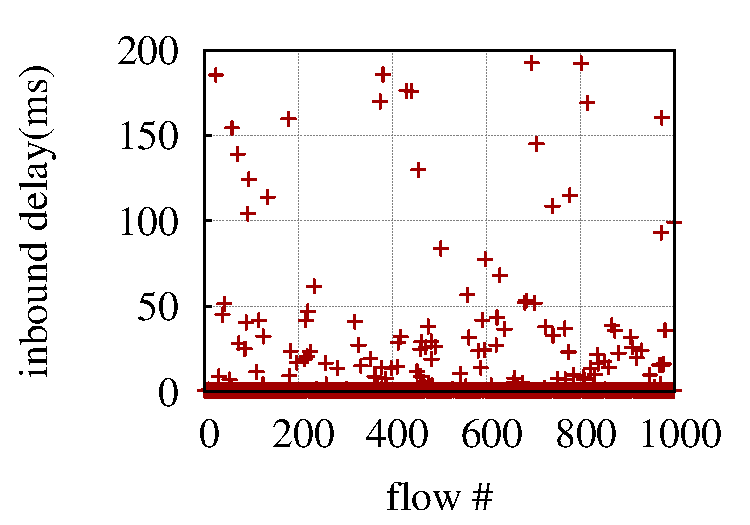
\includegraphics[width=\textwidth]{./figures/mazu/jan27_intel_inbound_with_pktout_flowmod_rate200-eps-converted-to.pdf}
	\caption{with flow\_mod/pkt\_out}
	\label{fig:intel_inbound_test3}
	\end{subfigure}
	\centering
        \begin{subfigure}[b]{0.40\textwidth}
        \centering
	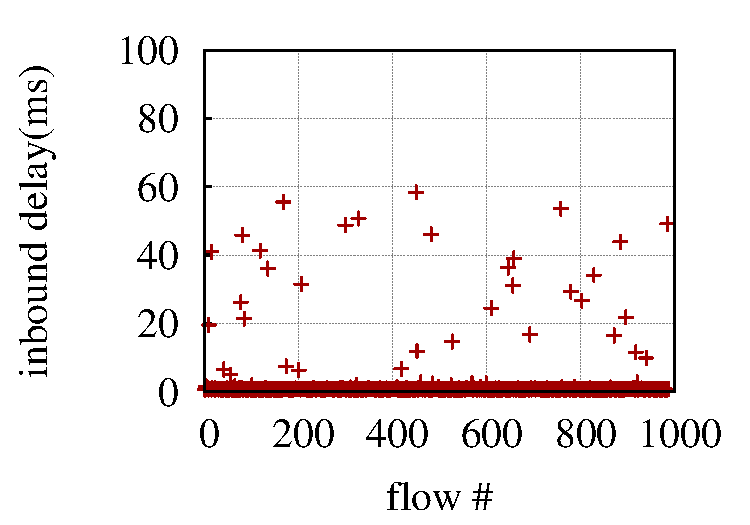
\includegraphics[width=\textwidth]{./figures/mazu/jan27_intel_inbound_wo_pktout_flowmod-eps-converted-to.pdf}
	\caption{w/o flow\_mod/pkt\_out}
	\label{fig:intel_inbound_test3_wo}
	\end{subfigure}	
	\caption{{\bf Inbound delay} on {\bf \Intel}, flow arrival rate = 200/s} 
	\label{fig:inbound-1}
\end{figure*}

To measure inbound latency, we empty the table at the switch, and we generate
traffic such that \packetin events are generated at a certain rate (i.e., we
create packets for new flows at a fixed rate). To isolate the impact of
\packetin processing from other message processing, we perform two kinds of
experiments: (1) the \packetin will trigger corresponding \flowmod (insert
simple OpenFlow rules differing just in destination IP) and \packetout
messages; (2) the\linebreak \packetin message is dropped silently by the
controller. 

We record the timestamp ($t_1$) when each packet is transmitted on the
measurement host's eth1 interface (\figref{mazu_experiment_setup}). We also record
the timestamp ($t_2$) when the host receives the corresponding \packetin
message on eth0. The difference ($t_2 - t_1$) is the inbound
latency.\footnote{Our technique differs from \cite{huang2013high}, where the
delay was captured from the switch to the controller, which includes
controller overhead.}


\begin{table}
\centering
\begin{scriptsize}
\begin{tabular}{cc}
\begin{tabular}{|c|c|c|}
\hline
\multicolumn{3}{|c|}{with flow mod/pkt out} \\ \hline
flow rate & 100/s  & 200/s  \\ \hline
cpu usage & 15.7\%    & 26.5\%   \\ \hline
\end{tabular}
&
\begin{tabular}{|c|c|c|}
\hline
\multicolumn{3}{|c|}{w/o flow mod/pkt out} \\ \hline
flow rate & 100/s   & 200/s \\ \hline
cpu usage & 9.8\%     & 14.4\%   \\ \hline
\end{tabular}
\end{tabular}
\caption{CPU usage on \Intel}
\label{fig:inbound-cpu}
\end{scriptsize}
\end{table} 

Representative results for an \Intel switch are shown in
\figref{fig:inbound-1};
\IBM has similar performance (5ms latency per \packetin on 
average).\footnote{\BroadcomOne and \BroadcomThree do not support \packetin
messages.} In the first experiment (\figref{fig:intel_inbound_test3}), we see the inbound latency is quite
variable with a mean of 8.33ms, a median of 0.73ms, and a standard deviation
of 31.34ms. In the second experiment (\figref{fig:intel_inbound_test3_wo}), the inbound delay is lower (mean of 
1.72ms, median of 0.67ms) and less variable (standard deviation of 6.09ms). 
We also observe that inbound latency depends on the \packetin rate: e.g. in
the first experiment the mean is 3.32 ms for 100 flows/s (not shown) vs. 8.33ms
for 200 flows/s (\figref{fig:intel_inbound_test3}).

The only difference between the two experiments is that in the former case
the switch CPU must process \flowmod and \packetout messages, and send
forwarding entries and outbound packets across the PCIe bus to the ASIC, in
addition to generating \packetin messages. As such, we observe that the CPU
usage is higher when the switch is handling concurrent OpenFlow operations and
generating more \packetin messages (\tabref{fig:inbound-cpu}). However, since
the Intel switch features a powerful CPU (\tabref{switch_para}), plenty of
CPU capacity remains. Our conversations with the switch vendor suggest that
the limited bus bandwidth between the ASIC and switch CPU is the primary
factor contributing to inbound latency. 

 
